\documentclass[a4paper]{scrartcl}

\usepackage[
    fancytheorems, 
    fancyproofs, 
    noindent, 
]{adam}


\title{Linear Algebra}
\author{Adam Kelly (\texttt{ak2316@cam.ac.uk})}
\date{\today}

\allowdisplaybreaks

\begin{document}

\maketitle

% This is a short description of the course. It should give a little flavour of what the course is about, and what will be roughly covered in the notes.

This article constitutes my notes for the `Linear Algebra' course, held in Michaelmas 2021 at Cambridge. These notes are \emph{not a transcription of the lectures}, and differ significantly in quite a few areas. Still, all lectured material should be covered. As a warning, this course has lots of results which involve just checking that a definition holds -- such proofs have been intentionally omitted.


\tableofcontents

\section{Vector Spaces}

\subsection{Vector Spaces and Subspaces}

Linear algebra is, somewhat obviously, primarily about studying objects that are \emph{linear} in nature. The objects we really care about are \emph{vector spaces}, settings in which we can add elements and multiply by scalars. We are also going to consider \emph{linear maps}, functions on vector spaces which preserve that linear structure -- but more on that later. 

Throughout the following discussion (and this course), $\F$ is going to denote an arbitrary field\footnote{A field $\F$ is a set $\F$ equipped with two operations $+$ (`addition') and $\cdot$ (`multiplication'). We require $\F$ with addition to form an abelian group, and multiplication must be associative and have an identity element $1$. We also require every element except $0$ to have an inverse with respect to multiplication, and multiplication must be distributive over addition.

Informally, you can think of a field as something you can do arithmetic in.}

\begin{definition}[$\F$-Vector Space ]
    An \vocab{$\F$-vector space} is an abelian group $(V, +)$ together with a function $\F \times V \rightarrow V$, written $(\lambda, v) \mapsto \lambda v$ such that the following axioms hold:
    \begin{enumerate}[label=(\roman*)]
        \item \emph{Distributivity in $V$}. $\lambda(v_1 + v_2) = \lambda v_1 + \lambda v_2$,
        \item \emph{Distributivity in $\F$}. $(\lambda_1 + \lambda_2)v = \lambda_1 v + \lambda_2 v$,
        \item \emph{Associativity}. $\lambda(\mu v) = (\lambda \mu) v$,
        \item \emph{Identity}. $1v = v$.
    \end{enumerate} 
\end{definition}

We usually call elements of $V$ \vocab{vectors} and elements of $\F$ \vocab{scalars}. The identity element in $V$ is usually called the zero vector, and is written $0_V$ (or just $0$ if the context is clear).

If $\F$ is $\R$ or $\C$, we use the terms `real vector space' and `complex vector space', since they're so common. 


\begin{example}[Examples of Vector Spaces]~
    \vspace{-1.5\baselineskip}
    \begin{enumerate}[label=(\roman*)]
        
        \item The set of triples
        $$
        \{(x, y, z) \mid x, y, z \in \R\}
        $$ 
        forms a real vector space called $\R^3$, because you can add any two triples component wise. 
        \item The set
        $$
        \Q[\sqrt{2}] = \{a + b\sqrt{2} \mid a, b \in \Q\}
        $$
        is a $\Q$-vector space, where we add elements and scale by rational numbers in the obvious way.
        \item The set $\mathcal{C}[0, 1]$ of all continuous functions $f: [0, 1] \rightarrow \R$ forms a real vector space.
    \end{enumerate}
\end{example}

As with many new objects, it's helpful to be able to discuss its substructure. In the case of a vector space $V$, there's a pretty natural notion for what it means for a subset $U \subseteq V$ to still act like a vector space.

\begin{definition}[Subspace]
    Let $V$ be a $\F$-vector space.
    A subset $U \subseteq V$ is a \vocab{subspace} of $V$ if $U$ is also an $\F$-vector space. If $U$ is a subspace of $V$, we will write $U \leq V$.
    
    % \begin{enumerate}[label=(\roman*)]
    %     \item $0 \in U$,
    %     \item $u_1, u_2 \in U$ implies that $u_1 + u_2 \in U$,
    %     \item $\lambda \in \F$, $u \in U$ implies that $\lambda u \in U$.
    % \end{enumerate}
\end{definition}

\begin{example}[Examples of Subspaces]~
    \vspace{-1.5\baselineskip}
    \begin{enumerate}[label=(\roman*)]
        \item The set of vectors $\{(x, y, z) \mid x, y, z \in \R, x + y + z = 0\}$ is a subspace of $\R^3$.
        \item The set of polynomials with terms of even degree $\{ a_0 + a_2 x^2 + a_4 x^4 + \cdots + a_{2k} x^{2k} \mid \alpha_{2i} \in \R, k \in \N\}$ is a subspace of $\R[X]$, the vector space of polynomials with coefficients in $\R$.
    \end{enumerate}
\end{example}

As you would expect, checking that something is a subspace is usually easier than checking all of the axioms for a vector space. In particular, to check that $U$ is a subspace of an $\F$-vector space $V$, you can just check that the following hold:
\begin{itemize}
    \item \emph{Zero vector}\footnote{You may wonder why we need to check this when we already check that we are closed under scaling. To see why, notice that we still have to ensure $U$ is non-empty!}. $0_V \in U$,
    \item \emph{Closure under addition}. $u_1, u_2 \in U$ to imply $u_1 + u_2 \in U$,
    \item \emph{Closure under scaling}. $\lambda \in \F$ and $u \in U$ to imply $\lambda u \in U$.
\end{itemize}


There are various ways in which we can manipulate subspaces, for example we can take the intersection of two subspaces, and we will get back another subspace. 

\begin{proposition}[Intersecting Subspaces]
    Let $U, W \leq V$. Then $U \cap W \leq V$.
\end{proposition}
\begin{proof}
    Since $U$ and $V$ are both subspaces of $V$, we have $0_V \in U \cap V$, and also since they are both closed under addition and scaling, $u_1, u_2 \in U \cap W$ implies that $u_1 + u_2 \in U \cap W$, and $\lambda \in \F$ implies $\lambda u \in U\cap W$. Thus $U \cap W$ is a subspace of $V$. 
\end{proof}

However we can't manipulate subspaces however we want and expect magic. For example, the union of two subspaces is generally \emph{not} a subspace, as it is typically not closed under addition. In fact, the union is only ever a subspace if one of the subspaces is contained in the other.\footnote{There are some more exercises of this flavour on the example sheet.}

We can however try to `complete' the union so that it becomes a subspace.

\begin{definition}[Sum of Subspaces]
    Let $V$ be a vector space over $\F$, and let $U, W \leq V$. We define the \vocab{sum} of $U$ and $W$ to be the set
    $$
    U + W = \{u + w \mid u \in U, w \in W \}.
    $$
\end{definition}

This definition immediately forces $U + W \leq V$, and indeed it is the minimal such space (in that any subspace of $V$ containing both $U$ and $W$ must also contain $U + W$).

\subsection{Quotient Spaces}

Since a vector space $V$ forms an abelian group $(V, +)$, we are able to take the quotient by any subspace $U \leq V$. 

\begin{definition}[Quotient Space]
    Let $V$ an $\F$-vector space, and let $U \leq V$. The \vocab{quotient space} $V/U$ is the abelian group $V/U$ equipped with the scalar multiplication $F \times V/U \rightarrow V/U$ written $(\lambda, v + U) \mapsto \lambda v + U$.
\end{definition}

With this definition, we need to check that this scalar multiplication operation 
is well defined. Indeed, if $v_1 + U = v_2 + U$ then
\begin{align*}
    v_1 - v_2 &\in U \\
\implies \lambda(v_1 - v_2) &\in U \\
\implies \lambda v_1 + U &= \lambda v_2 + U \in V/U,
\end{align*}
so our operation is indeed well defined.

As you would expect, taking a quotient gives you back a vector space.

\begin{proposition}[Quotient Spaces are Vector Spaces]
    $V/U$ is an $\F$-vector space.
\end{proposition}
\begin{proof}[Proof Sketch]
    Check definitions (most properties are inherited from $V$ being a vector space).
\end{proof}

% \subsection{Spans, Linear Independence, and Steinitz Exchange Lemma}

\subsection{Basis and Dimension}

You are likely informally familiar with the idea of \emph{dimension}, a measure how much freedom exists in a system. Dimensionality is a rather natural concept with respect to vector spaces, but we will need to move through some technicalities to establish the results we want.

To discuss the amount of freedom, we first need a way to quantify what it means for a set of vectors to be independent from one another. This is the idea of \emph{linear independence}.


\begin{definition}[Linear Independence]
We say that $\{v_1, \dots, v_n\} \in V$ are \vocab{linearly independent} if
$$
\lambda_1 v_1 + \lambda_2 v_2 + \cdots + \lambda_n v_n = 0
$$
implies that $\lambda_1 = \cdots = \lambda_n = 0$.
\end{definition}

\begin{remark}
    For an infinite subset $S \subseteq V$, we say it's linearly independent if every finite subset is linearly independent.
\end{remark}

If a set of vectors is \emph{not} linearly independent, then there's some vector in that set that can be written as a linear combination of the others -- so it's not independent of them!

The next idea we need to pin down is being able to see if our set of vectors can `generate' the rest of our vector space. 


\begin{definition}[Span]
    Let $V$ be a vector space over $\F$, and let $S \subset V$. We define the \vocab{span} of $S$, $\langle S \rangle$ to be the set of finite combinations of elements of $S$.

    If $\langle S \rangle = V$, then we say $S$ is \vocab{spans} or \vocab{generates} $V$.
\end{definition}

\begin{remark}
    By convention, we also take $\langle \emptyset \rangle = \{ 0\}$. An equivalent definition is that $\langle S \rangle$ is the smallest subspace of $V$ that contains $S$.
\end{remark}

\begin{example}[Quadratic Polynomials]
    Let $V$ be the vector space of quadratic polynomials over $\R$, 
    $$V = \{ax^2 + bx + c \mid a, b, c \in \R\}.$$ 
    Then the subset $S \subseteq V$ with $S = \{1, x, x^2\}$ spans $V$.
\end{example}

% \begin{definition}[Finite Dimension]
%     Let $V$ be a vector space over $\F$. We say that $V$ is \vocab{finite dimensional} if it is spanned by a finite set.
% \end{definition}

% \begin{example}[Finite and Infinite Dimensional Vector Spaces]
%     The space $\R[X]$ of polynomials with coefficients in $\R$ is infinite dimensional, but the space $\R_n[X]$ of polynomials of degree at most $n$ is finite dimensional, and is spanned by the set $\{1, X, X^2, \dots, X^n\}$.
% \end{example}

% \begin{definition}[Linear Independence]
% We say that $\{v_1, \dots, v_n\} \in V$ are \vocab{linearly independent} if
% $$
% \lambda_1 v_1 + \lambda_2 v_2 + \cdots + \lambda_n v_n = 0
% $$
% implies that $\lambda_1 = \cdots = \lambda_n = 0$.
% \end{definition}

% If a set of vectors is \emph{not} linearly independent, then one of the vectors in the set can be written as a linear combination of the others. 

% \begin{remark}
%     If $\{v_1, \dots, v_n\}$ are linearly independent, then $v_i \neq 0$ for all $i$.
% \end{remark}

Putting these two concepts together gives us the idea of \emph{bases}, which are sets of linearly independent vectors that span a vector space.

\begin{definition}[Basis]
    A subset $S$ of a vector space $V$ is a \vocab{basis} if $S$ is a set of linearly independent vectors that span $V$.
\end{definition}

\begin{example}[Basis for $\R^n$]
    The \vocab{canonical basis} of $\R^n$ is the set of vectors
    $$
    S = \left\{
        \begin{pmatrix}1 \\ 0 \\ \vdots \\ 0\end{pmatrix},
        \begin{pmatrix}0 \\ 1 \\ \vdots \\ 0\end{pmatrix},
        \dots,
        \begin{pmatrix}0 \\ 0 \\ \vdots \\ 1\end{pmatrix}
    \right\}.
    $$
    Importantly, this is not the \emph{only} basis of $\R^n$, just one that is quite convenient most of the time.
\end{example}

\begin{remark}
    Note that in the definition of a basis there is no requirement for the set of basis vectors $S \subseteq V$ to be finite -- only that any element in $V$ must be representable using finitely many elements of $S$. 
\end{remark}

We'd intuitively want to say that the \emph{dimension} of a vector space is the number of elements in its basis. However, we first need to check that this is a well defined notion.
We can at this point distinguish between finite and infinite dimensional vector spaces at this point though\footnote{Can you see why this is well defined already?}.

\begin{definition}[Finite \& Infinite Dimension]
    We say a vector space $V$ is \vocab{finite dimensional} if it has a finite basis, and we say it is \vocab{infinite dimensional} otherwise.
\end{definition}

The next result about bases we will prove is that they induce \emph{unique} representations of elements in the vector space.

\begin{lemma}[Unique Representations with a Basis]
    Let $V$ be a vector space over $\F$. Then $S \subseteq V$ is a basis of $V$ if and only if any vector $v \in V$ can be written uniquely as a linear combination of elements $v_1, \dots, v_n \in S$.
\end{lemma}
\begin{proof}
    Suppose that $S$ was a basis for $V$.
    Then if $v \in V$ can't be written as such a linear combination, then $S$ wouldn't not span $V$, contradicting it being a basis.
    Also, if $v$ can be written as such a linear combination non-uniquely, then taking
    $$
v = \lambda_1 v_1 + \cdots + \lambda_n v_n = \mu_1 v_1 + \cdots + \mu_n v_n.
    $$
    where $\lambda_i \neq \mu_i$ for at least one value of $i$, we'd have
    $0 = v - v = (\lambda_1 - \mu_1) v_1 + \cdots + (\lambda_n - \mu_n)v_n$,
    and at least one of these coefficients must be non-zero, contradicting $S$ being linearly independent.

    Alternatively, if any element in $V$ \emph{can} be written uniquely, then if $v_1, \dots, v_n \in S$ with $\lambda_1 v_1 + \cdots \lambda_n v_n = 0$ implies that $\lambda_1 = \cdots = \lambda_n = 0$, giving that $S$ must be linearly independent. Since $S$ is also spanning by definition, we see that it therefore must be a basis of $V$.
\end{proof}

With that out of the way, we can prove some results about finite dimensional vector spaces which will help us get towards our definition of dimension. 

\begin{lemma}[Spanning Sets Contain a Basis]
    Let $V$ be a finite dimensional vector space, and let $S = \{v_1, \dots, v_n\}$ be a set of vectors that spans $V$. Then there is some subset of $S$ that is a basis of $V$.
\end{lemma}
\begin{proof}
    If $\{v_1, \dots, v_n\}$ is linearly independent, then we are done. If it's not, then (up to reordering) we have $v_n \in \langle\{v_1, \dots, v_{n - 1}\}\rangle$. But then $\langle\{v_1, \dots, v_n\}\rangle = \langle\{v_1, \dots, v_{n - 1}\}\rangle$, so we can not include $v_n$ in our subset. Not including elements in this way repeatedly, since there is finitely many elements in $S$, we must eventually get a linearly independent set that still spans $V$.
\end{proof}

\begin{theorem}[Steinitz Exchange Lemma]
    Let $V$ be a finite dimensional vector space. Then if $\{v_1, \dots, v_m\}$ is a set of linearly independent vectors, and $\{w_1, \dots, w_n\}$ spans $V$, then
    \begin{enumerate}[label=(\roman*)]
        \item $m \leq n$
        \item up to reordering, $\{v_1, \dots, v_m, w_{m + 1}, \dots, v_n\}$ spans $V$.
    \end{enumerate}
\end{theorem}
\begin{proof}
    We will prove this by induction. Suppose we have replaced $\ell \geq 0$ of the $w_i$, and that
    $$
    \langle \{ v_1, \dots, v_\ell, w_{\ell + 1}, \dots, w_n\}\rangle = V.
    $$
    If $m = \ell$, we are done, so assume that $\ell < m$. Then since this set is spanning, we can write $v_{\ell + 1} \in V$ as
    $$
    v_{\ell+1} = \alpha_1 v_1 + \cdots + \alpha_{\ell} v_{\ell} + \beta_{\ell + 1} w_{\ell + 1} + \cdots + \beta_n w_n.
    $$ 
    Since having $\beta_i = 0$ for all $\ell + 1 \leq i \leq n$ would violate linear independence, we can suppose without loss of generality that $\beta_{\ell + 1} \neq 0$. We also note that this implies that $\ell + 1 \leq n$, as otherwise this would not be possible.

    Then $w_{\ell + 1} \in \langle \{v_1, \dots, v_{\ell + 1}, w_{\ell + 2}, \dots, w_{n} \} \rangle$, and this set spans $V$.

    Repeating this process, we will be done after $m$ steps, and we have also shown (at the final step) that $m \leq n$.
\end{proof}

\begin{corollary}[Dimension]
    Let $V$ be a finite dimensional vector space over $\F$. Then any two bases of $V$ have the same number of elements, called the \vocab{dimension} of $V$, denoted $\dim V$ or $\dim_\F V$.
\end{corollary}
\begin{proof}
    Immediate by Steinitz exchange lemma.
\end{proof}

So using Steinitz exchange lemma we have finally been able to pin down exactly what is meant by the dimension of a vector space -- it's the size of it's basis.
This should match up to the intuitive idea of `freedom' that you had at the start of this section. Freedom in a vector space comes from varying coefficients, and in a basis we can both freely vary coefficients and also reach any element in a vector space uniquely, so the number of independent parameters really is the size of the basis.

Steinitz also gives us a few useful results for free.

\begin{corollary}
    Let $V$ be a vector space over $\F$ with finite dimension $n = \dim V$. Then
    \begin{enumerate}[label=(\roman*)]
        \item Any independent set of vectors has at most $n$ elements, with equality if and only if it's a basis.
        \item Any spanning set has at least $n$ elements, with equality if and only if it's a basis.
    \end{enumerate} 
\end{corollary}
\begin{proof}
    Immediate by Steinitz exchange lemma.
\end{proof}

Working with basis and dimension can make the study of vector spaces much easier. For example, Steinitz allows us nicely extend bases. That is,
\begin{center}
	\color{blue}
    If we have a vector space $V$, and a subspace $U \leq V$, \\then we can pick a nice basis $\{u_1, \dots, u_\ell\}$ of $U$, and \\extend it to a basis $\{u_1, \dots, u_{\ell}, u_{\ell + 1}, \dots, u_n\}$ of $V$.
\end{center}Working with ideas like this can make many results easier to prove, as we will see in the following propositions.


\begin{proposition}[Dimension of the Sum of Subspaces]
    Let $U$, $W$ be subspaces of a vector space $V$. if $U$ and $W$ are finite dimensional, then so is $U + W$, and $\dim U + W = \dim U + \dim W - \dim U \cap W$.
\end{proposition}
\begin{proof}
    Pick a basis $\{v_1, \dots, v_a\}$ of $U \cap W$, and extend by Steinitz exchange lemma to a basis $\{v_1, \dots, v_a, u_1, \dots, u_b\}$ of $U$, and to a basis $\{v_1, \dots, v_a, w_1, \dots, w_c\}$ of $W$.
    
    It suffices to prove that $\{v_1, \dots, v_a, u_1, \dots, u_b, w_1, \dots, w_c\}$ is a basis of $U + W$.

    Clearly this set of vectors spans $U + W$, so we just need to check that they are linearly independent. Suppose that
    $$
    \sum_{i = 1}^{a} \alpha_i v_i + \sum_{i = 1}^b \beta_i u_i + \sum_{i = 1}^c \gamma_i w_i = 0.
    $$
    Rewriting,
    \begin{equation}\label{eq:thing}
        \sum_{i = 1}^{a} \alpha_i v_i + \sum_{i = 1}^b \beta_i u_i = -\sum_{i = 1}^c \gamma_i w_i, \tag{$\dagger$}
    \end{equation}
    where the LHS is in $U$ and the RHS is in $W$. This implies that
    $
    \sum_{i = 1}^c \gamma_i w_i \in U \cap W,
    $
    and can be written as 
    $
    \sum_{i = 1}^c \gamma_i w_i = \sum_{i = 1}^a  \mu_i v_i$,
    for some $\mu_i$, and then substituting this back into \eqref{eq:thing},
    $$
    \sum_{i = 1}^a (\alpha_i + \mu_i) v_i + \sum_{i = 1}^b \beta_i u_i = 0
    $$
    which forces $\beta_i = 0$. A similar argument also gives $\gamma_i = 0$, which then finally forces $\alpha_i = 0$, since $\{v_1, \dots, v_a\}$ is a basis.
\end{proof}

\begin{proposition}[Dimension of the Quotient Space]
    If $V$ is a finite dimensional vector space over $\F$ and $U \subseteq V$, then $U$ and $V / U$ are also finite dimensional, and $\dim V = \dim U + \dim V / U$.
\end{proposition}
\begin{proof}
    Let $\{u_1, \dots, u_\ell\}$ be a basis of $U$, and extend it via Steinitz exchange lemma to a basis $\{u_1, \dots, u_\ell, w_{\ell+1}, \dots, w_n\}$ of $V$.

    It's easy to see that $\{w_{\ell + 1} + U, \dots, w_{n} + U\}$ is a basis of $V/U$, as it clearly spans and linear independence is inherited from it being a basis of $V$. The result then follows.
\end{proof}

\subsection{Direct Sums}

Previously, we were able to look at the substructure of a vector space by looking at subspaces. Given two subspaces, we were then able to construct their sum, which is the set of all linear combinations of elements in each subspace. 

When studying a vector space using its subspaces in this way (considering their sum), it can be useful to impose an \emph{additional} constraint about the way in which the subspaces interact. In particular, it can be useful to impose a uniqueness constraint on the linear combinations that are created.

\begin{definition}[Direct Sum]
    Let $V$ be a vector space over $\F$, and let $U, W \leq V$. We say that $V$ is the \vocab{direct sum} of $U$ and $W$, written $V = U \oplus W$ if and only if every element $v \in V$ can be decomposed as
    $$
    v = u + w
    $$
    with $u \in U$ and $w \in W$, with this decomposition being unique.
\end{definition}

Of course, we can generalize the notion of a direct sum naturally to the case of multiple subspaces, in the way that you would expect.

\begin{remark}[Warning]
    We say that $W$ is \emph{a} direct complement of $U$ in $V$. There is \emph{no uniqueness} of such a complement!
\end{remark}



\begin{lemma}
    Let $V$ be a vector space and let $U, W \leq V$.
    Then the following are equivalent.
    \begin{enumerate}[label=(\roman*)]
        \item $V = U \oplus W$
        \item $V = U + W$ and $U \cap W = \{0\}$
        \item For any basis $B_1$ of $U$ and $B_2$ of $W$, the union $B = B_1 \cup B_2$ is a basis of $V$.
    \end{enumerate}
\end{lemma}
\begin{proof}
    \emph{(ii) implies (i)}. Let $V = U + W$ with $U \cap W = \{0\}$. Then for all $v \in V$, we can write $v = u + w$ with $u \in U$ and $w \in W$. To see that this is unique, suppose that
    $$
    v = u + w = u' + w'.
    $$
    Then $(u - u') = - (w-w')$, and thus they are both in $U \cap W$, but the only element of this is $0$, and thus $u = u'$ and $w = w'$, giving us uniqueness.

    \emph{(i) implies (iii)}. Let $B_1$ be a basis of $U$ and $B_2$ be a basis of $W$. Then $B = B_1 \cup B_2$ clearly spans $V$, so we need to check that it's linearly independent. Indeed, if
    $$
    \sum_{u \in B_1} \lambda_u u + \sum_{w \in B_2} \lambda_w w = 0,
    $$
    then $V = U \oplus W$ implies that since this is the sum of an element of $U$ and an element of $W$, then each is zero, and linear independence follows from $B_1, B_2$ being sets of linearly independent vectors.

    \emph{(iii) implies (ii)}. 
    Clearly we have $V = U+W$, so we just need to check that $U \cap W = \{0\}$. Let $v \in U \cap W$. Then we can write
    $$
    v = \sum_{u \in B_1} \lambda_u u = \sum_{w \in B_2} \lambda_w w \implies \sum_{u \in B_1} \lambda_u u - \sum_{w \in B_2} \lambda_w W = 0,
    $$
    and since $B_1 \cup B_2$ is a basis for $V$, we must have $\lambda_u, \lambda_w = 0$ for all $u, w \in B_1, B_2$, implying that $v = 0$.
\end{proof}

This result extends as you would expect for the case of direct products using multiple subspaces.

\section{Linear Maps}

\subsection{Linear Maps and Isomorphisms}

We are now going to turn our attention to \emph{linear maps}, which are maps that preserve the underlying structure of the vector space that they act on.

\begin{definition}[Linear Map]
    Let $V, W$ are vector spaces over $\F$.
    A map $\alpha: V \rightarrow W$ is a \vocab{linear map} if for all $\lambda_1, \lambda_2 \in \F$ and $v_1, v_2 \in V$ we have 
    $$
    \alpha(\lambda_1 v_1 + \lambda_2 v_2) = \lambda_1\alpha(v_1) + \lambda_2 \alpha(v_2).
    $$
\end{definition}

\begin{example}[Examples of Linear Maps]~
    \vspace{-1.5\baselineskip}
    \begin{enumerate}[label=(\roman*)]
        \item Consider the vector space $\mathcal{C}[0, 1]$ of continuous functions $f:[0, 1] \rightarrow \R$, Then for any fixed point $x \in [0, 1]$, the map $\alpha: C[0, 1] \rightarrow \R$ with $\alpha(f) = f(x)$ is a linear map.
        \item The map $\R^3 \rightarrow \R$ given by $(a, b, c) \mapsto 4a + 2b + c$ is a linear map.
        \item The map $\alpha: Q[\sqrt{2}] \rightarrow Q[\sqrt{2}]$ of `multiplying by $\sqrt{2}$' is a linear map, with $a + b \sqrt{2} \mapsto 2b + a \sqrt{2}$.
    \end{enumerate}
\end{example}

It's easy to see that the identity map is a linear map, and also that linearity is preserved by composing linear maps.

One nice thing about linear maps is that they interact well with basis, because of linearity. Indeed, specifying a linear map on the basis is sufficient to define that map on all of a vector space.

\begin{lemma}[Extension by Linearity]\label{lemma:extend-map}
    Let $V$ and $W$ be vector spaces, and let $B$ be a basis for $V$. Then if $\alpha_0: B \rightarrow W$ is \emph{any} map, then there exists a \emph{unique} linear map $\alpha: V \rightarrow W$ extending $\alpha_0$, so that for all $v \in B$ we have $\alpha(v) = \alpha_0(v)$.
\end{lemma}
\begin{proof}
    For $v \in V$, let $v = \sum_{i = 1}^n \lambda_i v_i$. Then necessarily by linearity, we define
    $$
    \alpha(v) = \alpha\left(\sum_{i = 1}^n \lambda_i v_i\right) = \sum_{i = 1}^n \lambda_i \alpha_0 (v_i).
    $$
    By construction this is a linear map and it extends $\alpha_0$.
\end{proof}

As with many other areas of pure mathematics, we have a special case for the structure preserving bijections on a given object.

\begin{definition}[Isomorphism]
    If $V$ and $W$ are vector spaces over $\F$, the linear map $\alpha: V \rightarrow W$ is an \vocab{isomorphism} if it also bijective. We say two vector spaces $V$ and $W$ are \vocab{isomorphic}, written $V \cong W$, if there is an isomorphism between them.
\end{definition}

\begin{remark}
    if $\alpha:V \rightarrow W$ is an isomorphism, then the inverse map $\alpha^{-1}$ exists and importantly it's \emph{also} linear.
\end{remark}

\begin{lemma}[Isomorphism is an Equivalence Relation]
    $\cong$ is an equivalence relation on the class of all vector spaces over $\F$.
\end{lemma}
\begin{proof}
    For reflexivity, we note that the identity map $id: V \rightarrow V$ is an isomorphism. For symmetry, we note that if $\alpha: V \rightarrow W$ is an isomorphism, then $\alpha^{-1}: W \rightarrow V$ is also an isomorphism. Lastly, we get transitivity because if $\alpha: U \rightarrow V$ and $\beta: V \rightarrow W$ are isomorphisms, then $\beta \circ \alpha: U \rightarrow W$ is also an isomorphism.
\end{proof}

From one perspective, isomorphism allows us to know when two objects are really just different representations of the same thing. With this in mind, the following result tells us something interesting (yet unsurprising) about the nature of finite dimensional vector spaces.


\begin{theorem}[Isomorphism for Finite Dimensional Vector Spaces]
    If $V$ is an $n$ dimensional vector space over $\F$, then $V \cong \F^n$, the vector space
    $$
    \F^n = \left\{\begin{pmatrix}x_1 \\ x_2 \\ \vdots \\ x_n\end{pmatrix} \mid x_1, \dots, x_n \in \F \right\},
    $$
    where addition is component-wise.
\end{theorem}
\begin{proof}
    Let $B = \{v_1, \dots, v_n\}$ be a basis for $V$. Then we claim that the map $\alpha: V \rightarrow \F^n$ defined by 
    $$
    v = \sum_{i = 1}^n \lambda_i v_i \longmapsto \begin{pmatrix}\lambda_1 \\ \vdots \\ \lambda_n\end{pmatrix}
    $$
    is an isomorphism. Indeed, it's easy to see that we have linearity inherited from $\F$, and also the map is a bijection, so indeed we do have $V \cong \F^n$.
\end{proof}

In particular, this result tells us that when we choose a basis for a finite dimensional vector space $V$, it's really the same as picking some isomorphism from $V$ to $\F^n$. 

This theorem also directly implies (with isomorphism being an equivalence relation) a criterion for two finite dimensional vector spaces to be isomorphic.

\begin{theorem}[Isomorphism Criterion]
    Let $V$ and $W$ be finite dimensional vector spaces over $\F$. Then they are isomorphic if and only if they have the same dimension.
\end{theorem}

\subsection{Images and Kernels}

Stepping back from isomorphisms, we need to define some frequently used concepts relating to linear maps.

\begin{definition}
    Let $V, W$ be vector spaces over $F$, and let $\alpha: V \rightarrow W$ be a linear map. We define the \vocab{kernel} of $\alpha$ as
    $$
    \kernel \alpha = \{ v\in V \mid \alpha(v) = 0\},
    $$
    and the \vocab{image} of $\alpha$ as
    $$
    \image \alpha = \{ w \in W \mid w = \alpha(v), v \in V\}.
    $$
\end{definition}

The structure of a linear map carries over to the image and the kernel, and naturally implies that they are both subspaces of their parent vector spaces.

\begin{lemma}[Image and Kernel are Subspaces]
    Let $\alpha: V \rightarrow W$ be a linear map. Then $\kernel \alpha$ and $\image \alpha$ are subspaces of $V$ and $W$ respectively.
\end{lemma}
\begin{proof}[Proof Sketch]
    Check definitions.
\end{proof}

You may recognize the definitions of the kernel and image from a course in group theory, particularly in relation to the first isomorphism theorem\footnote{Recall that if $G$ and $H$ are groups, and $\phi: G \rightarrow H$ is a homomorphism, then $G/\kernel{\phi} \cong \image \phi$.}. Indeed, remembering that vector spaces with vector addition are groups, with we can use the kernel and image of a linear map to establish an isomorphism between vector spaces.

\begin{theorem}[First Isomorphism Theorem For Vector Spaces]
    Let $V$ and $W$ be $\F$ vector spaces, and let $\alpha: V \rightarrow W$ be a linear map. Then $V/\kernel \alpha \cong \image \alpha$.
\end{theorem}
\begin{proof}[Proof Sketch]
    Consider the isomorphism $\overline{\alpha} : V/\kernel \alpha \rightarrow \image \alpha$ defined by $\overline{\alpha}(v + \kernel \alpha) = \alpha(v)$, and check definitions.
\end{proof}

Now while the kernel and image being subspaces are rather straightforward, slightly more interesting is the \emph{dimension} of these subspaces. This is described by the \emph{rank-nullity theorem}.

\begin{definition}[Rank and Nullity]
    Let $\alpha$ be a linear map. Then the \vocab{rank} of $\alpha$, $r(\alpha) = \dim \image \alpha$, is the dimension of the image. The \vocab{nullity} of $\alpha$, $n(\alpha) = \dim \kernel \alpha$, is the dimension of the Kernel.
\end{definition}

\begin{theorem}[Rank-Nullity Theorem]
    Let $U$ and $V$ be vector spaces such that $U$ is finite dimensional.
    Let $\alpha: U \rightarrow V$ be a linear map. Then
    $$
    \dim U = r(\alpha) + n(\alpha).
    $$
\end{theorem}
\begin{proof}
    We know that $U/\kernel \alpha \cong \image \alpha$. Thus $\dim (U / \kernel \alpha) = \dim (\image \alpha)$, that is $\dim U - \dim \kernel \alpha = \dim \image \alpha$, or $\dim U = r(\alpha) + n(\alpha)$.
\end{proof}

This result has an important consequence which is incredibly useful for quickly checking if a map is an isomorphism.

\begin{lemma}[Characterisation of Isomorphism]
    Let $V$ and $W$ be vector spaces over $\F$ with \emph{equal finite dimension}. Then the following are equivalent: 
    \begin{enumerate}[label=(\roman*)]
        \item $\alpha$ is injective,
        \item $\alpha$ is surjective,
        \item $\alpha$ is an isomorphism.
    \end{enumerate}
\end{lemma}
\begin{proof}[Proof Sketch]
    Follows directly from the rank-nullity theorem.
\end{proof}

\subsection{Matrices}

When dealing with vector spaces, it's sometimes convenient to work with vector spaces in the abstract, and other times it's convenient to pick some nice basis which you can easily work with.
When dealing with linear maps $\alpha: V \rightarrow W$, it it can also be useful to work with bases. The way we do this is by introducing \emph{matrices}.

It's important to say that matrices are not the essence of linear algebra, and in may cases viewing the subject in this way will just give you the impression that linear algebra is an opaque subject. Instead, you should think of matrices as a nice representations of linear maps for which its easy to perform computations with.
With that said, let's talk about linear maps.

In this section, we are going to discuss linear maps between two vector spaces $V$ and $W$.

\begin{definition}[Space of Linear Maps]
    Let $V$ and $W$ be vector spaces over $\F$. We define
    $$
    \mathcal{L}(v, w) = \{\alpha: V \rightarrow W \mid \alpha \text{ is a linear map}\}.
    $$
\end{definition}

\begin{proposition}[Space of Linear Maps is a Vector Space]
    $\mathcal{L}(V, W)$ is a vector space over $\F$. Moreover, if $V$ and $W$ are finite dimensional, then
    $$
    \dim \mathcal{L}(V, W) = \dim V \cdot \dim W.
    $$
\end{proposition}
\begin{proof}[Proof Sketch]    
    To see that $\mathcal{L}(V, W)$ is a vector space, one just needs to check definitions. We will leave the proof of the dimension until later.
\end{proof}

Now, given some linear map $\alpha$, let's think about how we can represent this map with respect to a basis.
Suppose that we had a finite dimensional vector space $V$ with basis $\{v_1, \dots, v_m\}$, and a finite dimensional vector space $W$ with basis $\{w_1, \dots, w_n\}$, and suppose that we had some linear map $\alpha : V \rightarrow W$.

Given some $v \in V$, if we wanted to work out $\alpha(v)$, we can write express $v$ in the basis above, with
$$
\alpha(v) = \alpha\left(\sum_{i = 1}^m \lambda_i v_i\right) = \sum_{i = 1}^m \lambda_i \alpha(v_i).
$$
So, to compute what $\alpha(v)$ is for any $v \in V$, it suffices to know what $\alpha(v_1), \dots, \alpha(v_m)$ is. To specify what say $\alpha(v_1)$ is, we can use the above basis of $W$ and write
$$
\alpha(v_1) = a_{11} w_1 + a_{21} w_2 + \cdots + a_{n1} w_n,
$$
for some coefficients $a_{i1}$. Repeating this for $v_2, \dots, v_n$ then totally specifies the linear map $\alpha$.
These collection of coefficients can be put into a \emph{matrix}, which will then be a representation of $\alpha$ when coupled with the bases $\{v_i\}$ and $\{w_i\}$.


\begin{definition}[Matrix]
    An $n \times m$ \vocab{matrix} over $\F$ is an array with $n$ rows and $m$ columns, with entries in $\F$:
    $$
    A = \begin{pmatrix}
        a_{11} & a_{12} & \cdots & a_{1m} \\
        a_{21} & a_{22} & \cdots & a_{2m} \\
        \vdots&\vdots&\ddots &\vdots\\
        a_{n1} & a_{n2} & \cdots & a_{nm}
    \end{pmatrix}.
    $$
    We denote the set of $n \times m$ matrices over $\F$ by $\mathcal{M}_{n,m}(\F)$.
\end{definition}

\begin{proposition}[Vector Space of Matrices]
    $\mathcal{M}_{n, m}(\F)$ is an $\F$-vector space.
\end{proposition}
\begin{proof}[Proof Sketch]
    Taking addition entry-wise we can just check definitions.
\end{proof}

\begin{proposition}[Dimension of $\mathcal{M}_{n,m}(\F)$]
    $\dim \mathcal{M}_{m, n}(\F) = m \times n$.
\end{proposition}
\begin{proof}
    We define the \emph{elementary matrix} $E_{i, j}$ such that every entry is $0$ except for the $i, j$th entry, which is $1$.
    Then the set $\{E_{i, j} \mid 1 \leq i \leq m, 1 \leq j \leq n\}$ is clearly a basis, and has $n \times m$ elements.
\end{proof}

Following on from the discussion above, we can now write down how linear maps can be represented using matrices.

\begin{definition}[Matrix of $\alpha$ in the $B, C$ Basis]
    Let $\alpha: V \rightarrow W$ be a linear map, and let $B = \{v_1, \dots, v_m\}$ be a basis of $V$ and $C = \{w_1, \dots, w_n\}$ be a basis of $W$. Then we define the \vocab{matrix of $\alpha$} to be
    $$
    [\alpha]_{B, C} = \begin{pmatrix}
        | & | & & | \\
        [\alpha(v_1)]_C & [\alpha(v_2)]_C & \cdots & [\alpha(v_m)]_C \\
        | & | & & |
    \end{pmatrix} = \begin{pmatrix}
        a_{11} & a_{12} & \cdots & a_{1m} \\
        a_{21} & a_{22} & \cdots & a_{2m} \\
        \vdots&\vdots&\ddots &\vdots\\
        a_{n1} & a_{n2} & \cdots & a_{nm}
    \end{pmatrix},
    $$
    where $a_{ij}$ is the coefficient of $w_i$ in $\alpha(v_j)$.
\end{definition}
\begin{remark}[Notation]
    We use $[v]_C$ to denote the column vector representing the vector $v$ in the basis $C$.
\end{remark}


\begin{proposition}[Matrix Representation of Linear Maps]
    If $V$ and $W$ are vector spaces over $\F$ such that $\dim V = n$ and $\dim W = m$, then $\mathcal{L}(V, W) \cong \mathcal{M}_{m, n}(\F)$.
\end{proposition}
\begin{proof}
    Fix a basis $B, C$ of $V$ and $W$ respectively.
    Then consider the linear map
    $
    \theta: \mathcal{L}(V, W) \rightarrow \mathcal{M}_{m, n}(\F)
    $ given by $\alpha \mapsto [\alpha]_{B, C}$.

    This map is clearly linear, and it's also clearly a bijection thus it's an isomorphism and our result follows.
\end{proof}

\begin{remark}
    This implies that $\dim \mathcal{L}(L, W) = m \times n$.
\end{remark}


What's nice about matrices is that they make working with linear maps \emph{easy}. It's generally much easier to manipulate arbitrary matrices than it is to arbitrary linear maps (of course, this varies from case to case), and we will see this in the following set of computational results.

You should be familiar from previous courses with the notion of matrix multiplication.

\begin{definition}[Matrix Multiplication]
    Let $A = (a_{ij})$ be an $n \times p$ matrix, and $B = (b_{ij})$ 
    be an $p \times m$ matrix.
    Then their \vocab{product} $C = A\cdot B$ is an $n \times m$ matrix $C = (c_{ij})$, with
    $$
    c_{ij} = \sum_{k = 1}^p a_{ik}b_{kj}.
    $$
\end{definition}

We can use matrix multiplication in lots of nice ways.

\begin{lemma}[Evaluating Linear Maps]
    Let $\alpha: V \rightarrow W$ be a linear map, and let $B, C$ be bases for $V$ and $W$ respectively. Then if $v \in V$, we have
    $$
    [\alpha(v)]_C = [\alpha_{B,C}] \cdot [v]_B.
    $$
\end{lemma}
\begin{proof}
    Let $v \in V$, and let $v = \sum_{j = 1}^n \lambda_j v_j$. Then
    $$
    \alpha(v) = \sum_{j = 1}^n \lambda_j \alpha(v_j) = \sum_{j = 1}^n \lambda_j \sum_{i = 1}^m a_{ij} w_i = \sum_{i = 1}^m \left(\sum_{j = 1}^n a_{ij} \lambda_j\right) w_i,
    $$
    as required.
\end{proof}

\begin{lemma}[Composing Linear Maps]
    Let $\alpha: V \rightarrow W$ and $\beta: U \rightarrow V$ be linear maps. Then if $A, B, C$ are bases of $U, V$ and $W$ respectively, we have 
    $$
    [\alpha \circ \beta]_{A, C} = [\alpha]_{B, C} \cdot [\beta]_{A, B}.
    $$
\end{lemma}
\begin{proof}[Proof Sketch]
    Use the definition of matrix multiplication to check that this map corresponds to the correct thing.
\end{proof}


% \begin{example}
%     Let $V$ and $W$ be finite dimensional vector spaces.
%     Consider the linear map $\alpha: V \rightarrow W$, and suppose $Y \leq V$. Consider the image of $Y$ under $\alpha$, $\alpha(Y) = \{ \omega \in W \mid \omega = \alpha(y), y \in Y\}$.

%     Define the sets $B' = \{v_1, \dots, v_k\}$ and $B'' = \{v_{k + 1}, \dots, v_n\}$ such that the union of disjoint sets $B = B' \cup B''$ is a basis for $V$, and $B'$ is a basis of $Y$ (that is, we extend using Steinitz exchange lemma).
    
%     Similarity we define $C' = \{w_1, \dots, w_\ell\}$ and $C'' = \{w_{\ell + 1}, \dots, w_m\}$ such that the union of disjoint sets $C = C' \cup C''$ is a basis for $W$ and $C'$ is a basis for $\alpha(Y)$.

%     Then we have the matrix
%     $$ 
%     [\alpha]_{B, C} = \begin{pmatrix}
%         \alpha(v_1) & \cdots & \alpha(v_k) & \alpha(v_{k + 1}) & \cdots & \alpha(v_n)
%     \end{pmatrix},
%     $$
%     and this will look like the block matrix
%     $$
%     \left[\begin{array}{ c | c }
%         A & B \\
%         \hline
%         0 & C
%       \end{array}\right],
%     $$
%     where $A$ is $k \times \ell$.
% \end{example}

\subsection{Change of Basis and Equivalent Matrices}

Matrices represent a linear map with respect to a given basis, so a natural question is how do we rewrite a matrix in a different basis? That is, 
given two vector spaces $V, W$ and a linear map $\alpha: V \rightarrow W$, we want to take the matrix $[\alpha]_{B, C}$ and express it with respect to the basis $B', C'$. 

The way we do this is by introducing a \emph{change of basis} matrix.

\begin{definition}[Change of Basis Matrix]    
    The \vocab{change of basis} matrix from $B'$ to $B$ is the matrix
    $P = [I]_{B', B}$, where $I$ is the identity map.
\end{definition}
\begin{remark}
    $P$ is an invertible square matrix, and $P^{-1}$ is the change of basis matrix from $B$ to $B'$. 
\end{remark}

Given a vector represented in a basis $B$, the change of basis matrix allows that vector to be expressed in a different basis $B'$.

\begin{lemma}[Change of Basis for a Vector]
    Let $B$ and $B'$ be bases for a vector space $V$, and let $v \in V$. Then if $P$ is the change of basis matrix from $B'$ to $B$ we have
    $$
    [v]_{B} = P[v]_{B'}.
    $$
\end{lemma}
\begin{proof}
    We know that $P = [I]_{B', B}$, and so $[I(v)]_B = [I]_{B', B} [v]_B' = P[v]_{B'}$.
\end{proof}

Using this idea of change of basis matrices, we can express the matrix of a linear map with respect to another basis.

\begin{proposition}[Change of Basis Formula]
    Let $A = [\alpha]_{B, C}$ and $A' = [\alpha]_{B', C'}$, and let $P$ be the change of basis from $B'$ to $B$ and $Q$ be the change of basis matrix from $C'$ to $C$. Then
    $$
    A' = Q^{-1} AP.
    $$
\end{proposition}
\begin{proof}[Proof Sketch]
    Check definitions.
\end{proof}

\subsection{Equivalent Matrices}

A natural notion of equivalence comes from saying 
two matrices are equivalent if there is some choice of basis for which they represent the same linear map. Using the change of basis formula, we can pin down this notion exactly.

\begin{definition}[Equivalent Matrices]
    We say that two matrices $A, A' \in \mathcal{M}_{m, n}(\FF)$ are \vocab{equivalent} if $A' = Q^{-1}AP$ for some invertible matrices $Q \in \mathcal{M}_{m, m}(\F)$ and $P \in \mathcal{M}_{n, n}$.    
\end{definition}

It's easy to check that this definition gives us an equivalence relation, and indeed it turns out that the equivalence classes of matrices are remarkably straightforward.

\begin{proposition}[Natural Basis for Matrices]
    Let $V, W$ be vector spaces over $\F$, with $\dim V = n$ and $\dim W = m$. Let $\alpha: V \rightarrow W$ be a linear map, Then there exists a basis $B$ of $V$ and a basis $C$ of $W$ such that
    $$
    [\alpha]_{B, C} = \left(\begin{array}{ c | c }
        I_r & 0 \\
        \hline
        0 & 0
      \end{array}\right),
    $$
    where $r = r(\alpha)$ and $I_r$ is the $r \times r$ identity matrix.
\end{proposition}
\begin{proof}
    We first choose a basis $\{v_{r + 1}, \dots, v_n\}$ of $\kernel \alpha$, and extend it to a basis $B = \{v_1, \dots, v_n\}$ of $V$.
    We will first show that $\{\alpha(v_1), \dots, \alpha(v_r)\}$ is a basis of $\image \alpha$.

    To see that it's spanning, given $v \in V$ we can write
    $\alpha(v) = \alpha\left(\sum_{i = 1}^n \lambda_i v_i\right) = \sum_{i = 1}^n \lambda_i \alpha(v_i) = \sum_{i =1}^r \lambda_i \alpha(v_i),
    $
    since $\alpha(v_i) = 0$ for $i > r$.
    
    To see that we have linear independence, suppose that $\sum_{i = 1}^r \lambda_i \alpha(v_i) = 0$. Then we have
    $
\alpha\left(\sum_{i = 1}^r \lambda_i v_i\right) = 0$ implying that
$\sum_{i = 1}^r \lambda_i v_i \in \kernel \alpha$,
    and since the kernel is spanned by $\{v_{r + 1}, \dots, v_n\}$ and $\{v_1, \dots, v_n\}$ is a basis, we must have $\lambda_i = 0$, as required.

    We can now extend this basis to a basis $C = \{\alpha(v_1), \dots$, $\alpha(v_r), w_{r + 1}, \dots, w_m \}$ of $W$. Then we can express $\alpha$ as a matrix in the basis $B$ and $C$ as
    \begin{align*}
        [\alpha]_{B, C} &=
    \begin{pmatrix}
        | &  & | & | &  & |\\
        [\alpha(v_1)]_C & \cdots & [\alpha(v_r)]_C & [\alpha(v_{r + 1})]_C & \cdots & [\alpha(v_n)]_C \\
        | &  & | & | &  & |
    \end{pmatrix} \\
    &= \begin{pmatrix}
        | &  & | & | &  & |\\
        [\alpha(v_1)]_C & \cdots & [\alpha(v_r)]_C & [0]_C & \cdots & [0]_C \\
        | &  & | & | &  & |
    \end{pmatrix},
    \end{align*}
    and it can easily be seen that this matrix is of the form desired.
\end{proof}

This result gives us a clear criterion for the equivalence of matrices, and also gives us a lovely result which is useful for choosing a basis which works nicely with the matrix representation of a linear map.

\begin{corollary}[Matrix Equivalence Criterion]
    Two $m \times n$ matrices are equivalent if the linear maps they represent have the same rank.
\end{corollary}

The equivalence criterion above is great, but doesn't give us a very easy way to see what the rank of the underlying linear map is, without doing a large amount of work. What we really want is a way to get this rank directly from the matrix. We can do this by considering the \emph{column} and \emph{row rank} of a matrix (which as we will see are really the same notion).

\begin{definition}[Column and Row Rank]
    Let $A \in \mathcal{M}_{m, n}(\F)$. The \vocab{column rank} of $A$, $r(A)$, is the dimension of the subspace of $\F^m$ spanned by the column vectors of $A$.

    Similarity, the \vocab{row rank} is the dimension of the subspace spanned by the row vectors of $A$ (that is, it's the column rank of $A^T$).
\end{definition}

\begin{remark}
    If $\alpha$ is a linear map, represented by a matrix $A$ with respect to some basis, then $r(A) = r(\alpha)$, so column rank is the same as the rank.
\end{remark}

\begin{proposition}[Equivalence from Row Rank]
    Two matrices $A, A'$ are equivalent if and only if $r(A) = r(A')$.
\end{proposition}
\begin{proof}
    If they are equivalent, then they correspond to the same linear map $\alpha$, expressed in two different bases. So the column rank is $r(A) = r(A') = r(\alpha)$, and we are done.

    If $r(A) = r(A') = r$, then $A$ and $A'$ are both equivalent to
    $$
    \left(\begin{array}{ c | c }
        I_r & 0 \\
        \hline
        0 & 0
      \end{array}\right),
      $$
      and by transitivity of equivalent, we have $A$ and $A'$ equivalent.
\end{proof}

The distinction between column rank and row rank is really non-existent, as the following result shows. This also means that we can refer to the column and row rank as just the `rank' of the matrix.

\begin{theorem}[Column Rank Equals Row Rank]
    $r(A) = r(A^T)$
\end{theorem}
\begin{proof}
    Let $r = r(A)$. Then we know that 
    we can write
    $$
    Q^{-1}AP = \left(\begin{array}{ c | c }
        I_r & 0 \\
        \hline
        0 & 0
      \end{array}\right),
    $$
    then taking the transpose, we have $(Q^{-1}AP)^T = P^T A^T (Q^{-1})^T = P^T A^T (Q^T)^{-1}$
    so $P^T A^T (Q^T)^{-1}$ is 
    $$
    \left(\begin{array}{ c | c }
        I_r & 0 \\
        \hline
        0 & 0
      \end{array}\right)^T,
    $$
    which is an $n \times m$ matrix. But then $r = r(A) = r(A^T)$.
\end{proof}

Let's now consider the special case of \vocab{endomorhisms}, that is, linear maps $\alpha: V \rightarrow V$.

If $B$ and $B'$ are a basis for $V$, and $P$ is the change of basis matrix from $B'$ to $B$, then given $\alpha$ we have $[\alpha]_{B', B'} = P^{-1}[\alpha]_{B, B}P$, which is a special case of the change of basis formula.
This idea of writing a matrix using the same basis for the domain and range gives us \emph{similarity}, another notion of matrices being the same.

\begin{definition}[Similar Matrices]
    Let $A, A'$ be two $n \times n$ square matrices. We say that $A$ and $A'$ are \vocab{similar} or \vocab{conjugate} if and only if  $A' = P^{-1} A P$ for some invertible $n \times n$ matrix $P$.
\end{definition}

This idea of similarity will be a central concept when we deal with the diagonalization of such matrices later on.


\section{Dual Space}

\subsection{Defining the Dual Space}

We are now going to turn our attention to an interesting set of linear maps on a vector space.

\begin{definition}[Dual Space]
    Let $V$ be a vector space over a field $\F$. The \vocab{dual space} $V^*$ is the set of linear maps from $V$ to $\F$,
    $$
    V^* = \mathcal{L}(V, \F).
    $$
\end{definition}

So how should we understand this space?
As usual, things are easier for finite dimensional vector spaces, so we are going to start there. We know from the previous section that \emph{any} linear map is determined by its action on basis vectors. So if we have some finite dimensional vector space $V$ with basis $\{v_1, \dots, v_n\}$ and a linear map $\alpha: V \rightarrow \F$, we just need to know $\alpha(v_1), \dots, \alpha(v_n) \in \F$.

This tells us exactly what the nice way to think about the dual space is -- through a basis that just picks out basis vectors so that we can deal with them individually. We call this the \emph{dual basis}.\footnote{We just write it as a definition here, but we should really check that it is indeed a basis of the dual, but I think it's relatively clear so this is left to the reader.}

\begin{definition}[Dual Basis]
    Let $V$ be a finite dimensional vector space over $\F$ with a basis $B = \{v_1, \dots, v_n\}$. 
    Then we define the \vocab{dual basis} for $V^*$ to be $B^* = \{\varepsilon_1, \dots, \varepsilon_n\}$ where $\varepsilon_j(v_i) = \delta_{ij}$.

    In particular, if $v \in V$ can be written as $v = \sum_{i = 1}^n \lambda_i v_i$, then $\varepsilon_j(v) = \lambda_j$.
\end{definition}

Since this is a basis of $V^*$, we can immediately see that $\dim V^* = \dim V$. Sometimes it's also convenient to think of $V^*$ as the space of row vectors of length $m$ over $\F$\footnote{There's also a hidden inner product structure here, but we won't dwell on that.}

\subsection{The Annihilator}


When we have some subset $U$ of a vector space $V$, we frequently care about the set of linear maps that are zero on everything in $U$. This construction ends up gives us a subspace of the dual space $V^*$.


\begin{definition}[Annihilator]
    If $V$ is a vector space over $\F$, and $U \subseteq V$, then the \vocab{annihilator} of $U$ is the set $U^0$ of linear maps $V \rightarrow \F$ that are zero on $U$,
    $$
    U^0 = \{ \alpha \in V^* \mid \alpha(u) = 0 \text{ for all }u \in U\}.
    $$
\end{definition}

\begin{lemma}[Annihilator is a Subspace]
    The annihilator is always a subspace of the dual, that is, $U^0 \leq V^*$.
\end{lemma}
\begin{proof}[Proof Sketch]    
    Check definitions.
\end{proof}

By thinking about the annihilator, we also get a result that looks a little like rank-nullity.

\begin{lemma}[Rank-Nullity for the Annihilator]
    If $V$ is a finite dimensional vector space and $U \leq V$, then $\dim V = \dim U + \dim U^0$.
\end{lemma}
\begin{proof}[Proof Sketch]
    Let $\{v_1, \dots, v_k\}$ be a basis of $U$, and extend it to a basis $B = \{v_1, \dots, v_n\}$ of $V$. Then the dual basis is $B' = \{\varepsilon_1, \dots, \varepsilon_n\}$.
    We then just need to check that $\{\varepsilon_{k + 1}, \dots, \varepsilon_n\}$ is a basis of $U^0$.
\end{proof}

\subsection{The Dual Map}

We will now see that thinking about the dual will give us a basis-free interpretation of what corresponds with the transpose of a matrix.

\begin{definition}[Dual Map]
    Let $V$ and $W$ be vector spaces, and suppose that $\alpha: V \rightarrow W$ is a linear map. Then we define the \vocab{dual map} of $\alpha$ to be linear map $\alpha^*: W^* \rightarrow V*$ given by $\varepsilon \mapsto \varepsilon \circ \alpha$.
\end{definition}

To see what this is all about, consider the following example.

\begin{example}[Using the Dual Map]
Let $V$ and $W$ be $\R$ vector spaces, and let $B = \{v_1, v_2, v_3\}$ be a basis for $V$ and $C = \{w_1, w_2\}$ be a basis for $W$.

We define the linear map $\alpha: V \rightarrow W$ by
\begin{align*}
    \alpha(v_1) &= w_1 + w_2 \\
    \alpha(v_2) &= 2w_1 - w_2 \\
    \alpha(v_3) &= 6w_1 + 3w_2.
\end{align*}
Now we can see what the dual map $\alpha^*: W^* \rightarrow V^*$ looks like. Let $B^* = \{v_1^*, v_2^*, v_3^*\}$ be the corresponding dual basis of $V$, and let $C^* = \{w_1^*, w_2^*\}$ be the corresponding dual basis of $W$. Then for any $v = av_1 + bv_2 + cv_3$ we have
\begin{align*}
    [\alpha^*(w_1^*)](v) &= w_1^*(\alpha(av_1 + bv_2 + cv_3)) \\
    &= w_1^*((a + 2b + 6c)w_1 + (a - b + 3c)w_2)\\
    &= a + 2b + 6c,
\end{align*}
and in this way, we can really write
$$
\alpha^*(w_1^*) = v_1^* +  2v_2^* + 6v_3^*, \quad \text{and} \quad \alpha^*(w_2^*) = v_1^* - v_2^* + 3v_3^*,
$$
which totally specifies $\alpha^*$.
\end{example}

A slightly more interesting way of viewing this example is through the lense of matrices.

\begin{example}[Above with Matrices]
Continuing on from the example above, we can see that in the $B, C$ basis we have
$$
[\alpha]_{B, C} = \begin{pmatrix}
    1 & 2 & 6 \\
    1 & -1 & 3
\end{pmatrix}.
$$
Then $\alpha^*$ in the $C^*, B^*$ basis is given by
$$
[\alpha^*]_{C^*, B^*} = \begin{pmatrix}
    1 & 1 \\ 2 & -1 \\ 6 & 3
\end{pmatrix}.
$$
\end{example}

Of course, in finite dimensions this works in the general case.

\begin{theorem}[Transpose Interpretation of the Dual Map]
    Let $V$ and $W$ be finite dimensional vector spaces over $\F$. Let $B$ be a basis for $V$ and $C$ be a basis for $W$, and let $B^*, C^*$ be the corresponding dual spaces.
    Then if $\alpha: V \rightarrow W$ is a linear map, we have
    $$
    [\alpha^*]_{C^*, B^*} = [\alpha]_{B, C}^T.
    $$
\end{theorem}
\begin{proof}
    Let $B = \{v_1, \dots, v_n\}$ be a basis for $V$ and $C = \{w_1, \dots, w_m\}$ be a basis for $W$, and let $B^*, C^*$ be the corresponding dual spaces. Then 
    $$
    ([\alpha]_{B, C})_{i, j} = ([\alpha(v_i)]_{C})_j = ([w_j^* \circ \alpha]_{B^*})_i = ([\alpha^*]_{C^*, B^*})_{j, i},
    $$
    as required.
\end{proof}

This result about viewing the matrix of $\alpha^*$ in terms of the matrix of $\alpha$ hints at a more general perspective where it can be easier to understand one of $\alpha$ and it's dual $\alpha^*$ than the other, and indeed many properties of $\alpha^*$ can be derived from $\alpha$. 

For example, the result below is \emph{immensely important}\footnote{But we won't see in this course why that is.} and is an example of the `duality approach'. 

\begin{proposition}[Properties of the Dual Map]
    Let $V$ and $W$ be vector spaces over $\F$, and let $\alpha: V \rightarrow W$ be a linear map. Then
    \begin{enumerate}[label=(\roman*)]
        \item $\kernel \alpha^* = (\image \alpha)^0$, so $\alpha^*$ is injective if and only if $\alpha$ is surjective.
        \item $\image \alpha^* \leq (\kernel \alpha)^0$, with equality if $V$ and $W$ are finite dimensional (in this case, $\alpha^*$ is surjective if and only if $\alpha$ is injective).
    \end{enumerate}
\end{proposition}
\begin{proof}
    (i) Let $\varepsilon \in W^*$. Then $\varepsilon \in \kernel \alpha^*$ if and only if $\alpha^*(\varepsilon) = 0$, that is, if $\varepsilon(\alpha(v)) = 0$ for all $v \in V$. But this occurs if and only if $\varepsilon \in (\image \alpha)^0$.

    (ii) We will first show that $\image \alpha^* \leq (\kernel \alpha)^0$. Indeed, let $\varepsilon \in \image \alpha^*$. Then $\varepsilon = \alpha^*(\phi)$ for some $\phi \in W^*$. But then for all $u \in \kernel \alpha$ we have $\varepsilon (u) = (\alpha^*(\phi))(u) = \phi(\alpha(u)) = 0$. So then $\varepsilon \in (\kernel \alpha)^0$, and thus $\image \alpha^* \leq (\kernel \alpha)^0$ as required. 

    In finite dimensions, we can compute the dimensions of the two spaces. We have
    $$
    \dim \image \alpha^* = r(\alpha^*) = r([\alpha^*]_{C^*, B^*}) = r([\alpha]^T_{B, C}) = r(\alpha).
    $$
    So $\dim \image \alpha^* = r(\alpha)$, and by rank-nullity, this is $\dim V - \dim \kernel \alpha = \dim \; (\kernel \alpha)^0$. So $\image \alpha^* \leq (\kernel \alpha)^0$ and also $\dim \image \alpha^* = \dim (\kernel \alpha)^0$,  giving us equality.
\end{proof}

\subsection{Double Dual}

In general, there is no \emph{obvious} relation between $V$ and $V^*$, in that all of the relations we discussed in the previous section rely on choosing a basis -- and choosing bases is an inherently arbitrary process. However, there \emph{is} a canonical (that is, basis free) relation between $V$ and $(V^*)^*$.

\begin{definition}[Double Dual]
    Let $V$ be a vector space over $\F$, and $V^* = \mathcal{L}(V, \F)$ be the dual of $V$. Then we define the \vocab{double dual} or \vocab{bidual} of $V$ to be
    $$
    V^{**} = \mathcal{L}(V^*, \F) = (V^*)^*.
    $$
\end{definition}

Indeed, there is a \emph{canonical} embedding from $V$ to $V^{**}$, and there are non-trivial examples\footnote{Such as $L^P(\R^d) = \{f: \R^d \rightarrow \R \mid \int_{R^d} |f(x)|^{p} \dd x < \infty\}$.} of infinite dimensional spaces where $V \cong V^{**}$.

\begin{center}
    

\tikzset{every picture/.style={line width=0.75pt}} %set default line width to 0.75pt        

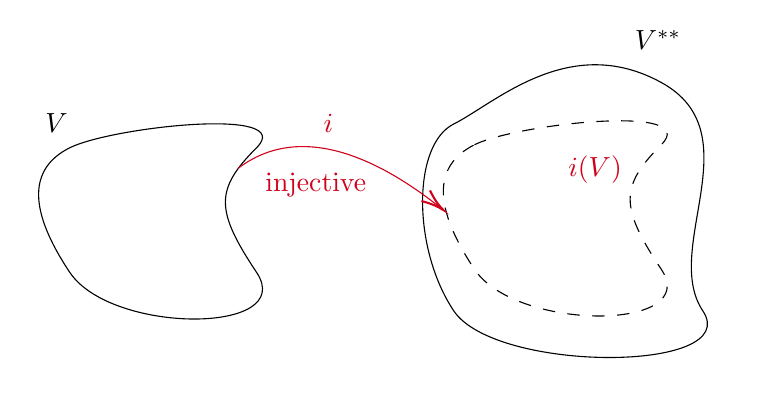
\begin{tikzpicture}[x=0.75pt,y=0.75pt,yscale=-1,xscale=1]
%uncomment if require: \path (0,421); %set diagram left start at 0, and has height of 421

%Shape: Polygon Curved [id:ds23351701075718778] 
\draw   (100,280) .. controls (120,270) and (210,260) .. (190,280) .. controls (170,300) and (170,310) .. (190,340) .. controls (210,370) and (120,370) .. (100,340) .. controls (80,310) and (80,290) .. (100,280) -- cycle ;
%Shape: Polygon Curved [id:ds5106655891262244] 
\draw  [dash pattern={on 4.5pt off 4.5pt}] (295,278.54) .. controls (315,268.54) and (405,258.54) .. (385,278.54) .. controls (365,298.54) and (365,308.54) .. (385,338.54) .. controls (405,368.54) and (315,368.54) .. (295,338.54) .. controls (275,308.54) and (275,288.54) .. (295,278.54) -- cycle ;
%Shape: Polygon Curved [id:ds3732810569342433] 
\draw   (285,268.54) .. controls (305,258.54) and (340.67,224.22) .. (385,248.54) .. controls (429.33,272.87) and (385,328.54) .. (405,358.54) .. controls (425,388.54) and (305,388.54) .. (285,358.54) .. controls (265,328.54) and (265,278.54) .. (285,268.54) -- cycle ;
%Curve Lines [id:da8915674336439121] 
\draw [color={rgb, 255:red, 208; green, 2; blue, 27 }  ,draw opacity=1 ]   (181,290) .. controls (212.85,265.71) and (252.46,287.99) .. (278.81,309.04) ;
\draw [shift={(280,310)}, rotate = 219] [color={rgb, 255:red, 208; green, 2; blue, 27 }  ,draw opacity=1 ][line width=0.75]    (10.93,-3.29) .. controls (6.95,-1.4) and (3.31,-0.3) .. (0,0) .. controls (3.31,0.3) and (6.95,1.4) .. (10.93,3.29)   ;

% Text Node
\draw (87,262.4) node [anchor=north west][inner sep=0.75pt]    {$V$};
% Text Node
\draw (371,222.4) node [anchor=north west][inner sep=0.75pt]    {$V^{**}$};
% Text Node
\draw (221,262.4) node [anchor=north west][inner sep=0.75pt]  [color={rgb, 255:red, 208; green, 2; blue, 27 }  ,opacity=1 ]  {$i$};
% Text Node
\draw (193,291) node [anchor=north west][inner sep=0.75pt]  [color={rgb, 255:red, 208; green, 2; blue, 27 }  ,opacity=1 ] [align=left] {injective};
% Text Node
\draw (339,282.4) node [anchor=north west][inner sep=0.75pt]  [color={rgb, 255:red, 208; green, 2; blue, 27 }  ,opacity=1 ]  {$i( V)$};


\end{tikzpicture}

\end{center}

This canonical embedding is described by `evaluating at $v$'.

\begin{theorem}[Canonical Embedding of $V$ into $V^{**}$]
    There is a natural injective linear map from $V$ to $V^{**}$, called the \vocab{evaluation map}.
\end{theorem}
\begin{proof}
Let $V$ be an $\F$ vector space, and let $v \in V$.
We define the evaluation at $v$ map
$$
\hat{v}: V^* \rightarrow \F \quad \text{by} \quad \hat{v}(\varepsilon) = \varepsilon(v).
$$
Then $\hat{v}(\varepsilon_1 + \lambda \varepsilon_2) = (\varepsilon_1 + \lambda \varepsilon_2)(v) = \varepsilon_1(v) + \lambda \varepsilon_2(v)$, so $\hat{v} \in V^{**}$.

The proof that this is injective is intentionally omitted.
\end{proof}


\begin{theorem}[Canonical Embedding in Finite Dimensions]
    If $V$ is finite dimensional, then the evaluation map is an isomorphism.
\end{theorem}
\begin{proof}
    We know that for $v \in V$ we have the evaluation map $\hat{v} \in V^{**}$. It's easy to see that the map $v \mapsto \hat{v}$ is linear in $v$, so it is left to check that this map is a bijection.

    Let $e \in V \backslash {0}$. We can extend $\{e\}$ to a basis $B = \{e, e_2, \dots, e_n\}$ of $V$. Let $B^*$ be the dual basis of $V$. 
    Then
    $$
    \hat{e}(e^*) = e^*(e) = 1,
    $$
    and in particular, $\hat{e} \neq 0$, so the kernel of the map $v \mapsto \hat{v}$ contains only $0$, and thus it is injective\footnote{This step of the proof has an analogue in infinite dimensions for a certain kind of vector space (Banach space), but requires the use of non-trivial results (the Hahn-Banach theorem).}.

    To see that this map is an isomorphism, we just need to compute dimensions. We know that $\dim V = \dim V^* = \dim (V^*)^* = \dim V^{**}$, and this along with injectivity implies that the map $v \mapsto \hat{v}$ is an isomorphism.
\end{proof}

This canonical embedding allows us to `identify' $V$ and $V^{**}$, which in turn can be used to prove various facts about say the annihilator.

\begin{lemma}[Double Annihilator]
    Let $V$ be a finite dimensional vector space over $\F$, and $U \leq V$. Then
    $\hat{U} = U^{00}$, so after identification of $V$ and $V^{**}$, we have $U = U^{00}$.
\end{lemma}
\begin{proof}
    Let us first show that $U \leq U^{00}$. Indeed, let $u \in U$. Then for all $\varepsilon \in U^0$, $\varepsilon(u) = 0$. But then $\varepsilon(u) = \hat{u}(\varepsilon) = 0$, so $\hat{u} \in U^{00}$, and $\hat{U} \leq U^{00}$.
    
    We can then compute dimensions, and $\dim U^{00} = \dim V - \dim U^{0} = \dim U$, and since $v \mapsto \hat{v}$ is an isomorphism, $\dim \hat{U} = 
    \dim U$. Thus $\dim \hat{U} = \dim U = \dim U^{00}$, and $\hat{U} = U^{00}$.
\end{proof}

\begin{remark}
    With the identification of $V^{**}$ and $V$, for $T \leq V^{*}$ we can define $T^0 = \{v \in V \mid \alpha(v) = 0, \; \forall \alpha \in T\}$.
\end{remark}

These results give us some unsurprising properties which are useful for doing computations.

\begin{lemma}[Sums and Intersections of Annihilators]
    Let $V$ be a finite dimensional vector space over $\F$, and let $U_1, U_2 \leq V$. Then 
    \begin{enumerate}[label=(\roman*)]
        \item $(U_1 + U_2)^0 = U_1^0 \cap U_2^0$;
        \item $(U_1 \cap U_2) = U_1^0 + U_2^0$.
    \end{enumerate}
\end{lemma}
\begin{proof}
    (i) Let $\theta \in V^*$, then $\theta \in (U_1 + U_2)^0$ if and only if $\theta(u_1 + u_2) = 0$ for all $u_1 \in U_1$ and $u_2 \in U_2$. By linearity this is exactly when $\theta(u) = 0$ for $u \in U_1 \cup U_2$, which occurs if and only if $\theta \in U_1^0 \cap U_2^0$.

    (ii) Take the annihilator of the result in (i), and use the fact that $U^{00} = U$.
\end{proof}

\section{Bilinear Forms}

\subsection{Introducing Bilinear Forms}

In the previous section we considered linear maps from a vector space to the scalar field that vector space is over. In this section we will look at a related but interesting set of maps which have \emph{two} arguments and are linear in both.
Such maps are \emph{bilinear forms}.

\begin{definition}[Bilinear Form]
    Let $U$ and $V$ be vector spaces over $\F$. Then $\phi: U \times V \rightarrow \F$ is a \vocab{bilinear form} if it is linear in both components.
\end{definition}

\begin{example}[Examples of Bilinear Forms]
    The following are all bilinear forms.
    \begin{enumerate}[label=(\roman*)]
        \item A canonical example -- the scalar product on $U = V = \R^n$.
        \item The map $V \times V^* \rightarrow \F$ given by $(v, \alpha) \mapsto \alpha(v)$.
        \item For $U = V = \mathcal{C}([0, 1],\R)$ the map
        $
        \phi(f, g) = \int_0^1 f(t) g(t) \dd t.
        $
    \end{enumerate}
\end{example}

There is a standard representation of bilinear forms using matrices.

\begin{definition}[Matrix of a Bilinear Form]
    Let $B = \{u_1, \dots, u_n\}$ be a basis of $U$ and $C = \{v_1, \dots, v_m\}$ be a basis of $V$, and let $\phi: U \times V \rightarrow \F$ be a bilinear form.
    
    We define the \vocab{matrix of $\phi$} with respect to $B$ and $C$ by
    $$
    ([\phi]_{B, C})_{i, j} = \phi(u_i, v_j). 
    $$
\end{definition}

\begin{lemma}[Evaluating a Bilinear Form]
    Let $\phi: U \times V \rightarrow \F$ be a bilinear form, and let $u \in U$ and $v \in V$. Then if $B$ is a basis of $U$ and $C$ is a basis of $V$, we have
    $$
    \phi(u, v) = [u]_B^T [\phi]_{B, C} [v]_C.
    $$
\end{lemma}
\begin{proof}[Proof Sketch]
    Check definitions.
\end{proof}

\begin{remark}
    $[\phi]_{B, C}$ is the unique matrix such that this equation holds.
\end{remark}

It's sometimes useful to study a bilinear form in just one of its arguments. This can be done by considering the induced maps.

\begin{definition}[Induced Map of a Bilinear Form]    
    Let $\phi: U \times V \rightarrow \F$ be a bilinear form. Then $\phi$ determines two linear maps $\phi_L: U \rightarrow V^*$ and $\phi_R: V\rightarrow U^*$, with
    $$
    (\phi_L(u))(v) = \phi(u, v) \quad \text{and} \quad (\phi_R(v))(u) = \phi(u, v).
    $$
\end{definition}

These induced maps area easily obtained from the matrix of the bilinear form.

\begin{lemma}[Matrices of the Induced Maps]
    Let $\phi: U \times V \rightarrow \F$ be a bilinear map.
    Then if $B = \{u_1, \dots, u_n\}$ is a basis of $U$ and $C = \{v_1, \dots, v_m\}$ is a basis of $U$, then if $A = [\phi]_{B, C}$ we have
    $$
    [\phi_R]_{C, B^*} = A \quad \text{and} \quad [\phi_L]_{B, C^*} = A^T.
    $$
\end{lemma}
\begin{proof}[Proof Sketch]
    Check definitions.
\end{proof}

\section{Lecture 14}

\subsection{Cramer's Rule}

We have an algorithm for computing the unique solution to $Ax = b$ without computing $A^{-1}$.

\begin{proposition}[Cramer's Rule]
    Let $A \in \mathcal{M}_{n , n}(\F)$ be an invertible matrix, and let $b \in \F^n$. Then the unique solution to $Ax = b$ is given by
    $$
    x_i = \frac{1}{\det A} \det(A_{\hat{ib}}),
    $$
    where $A_{\hat{i}b}$ is teh matrix obtained by replacing the $i$th column of $A$ by $b$.
\end{proposition}
\begin{proof}
    Since $A$ is invertible, there exists a unique $x \in \F^n$ with $Ax = b$. Then
    computing we have
    \begin{align*}
        \det(A_{\hat{ib}}) &= \det(A^{(1)}, \dots, A^{(i - 1)}, b, A^{(i + 1)}, A^{(n)}) \\
        &= \det(A^{(1)}, \dots, A^{(i - 1)}, Ax, A^{(i + 1)}, A^{(n)}) \\
        &= \det(A^{(1)}, \dots, A^{(i - 1)}, \sum_{j = 1}^n x_j A^{(j)}, A^{(i + 1)}, A^{(n)}) \\
        &= x_i \det(A^{(1)}, \dots, A^{(i - 1)}, A^{(i)}, A^{(i + 1)}, A^{(n)})  \\
        &= x_i \det A.
    \end{align*}
\end{proof}

\section{Diagonalization, Eigenvectors and Eigenvalues}


\subsection{Antidiagonal Matrices}

We are now going to take the first steps towards the diagonalisation of endomorphisms. 
Given a finite dimensional vector space $V$ over $\F$ and some endomorphism $\alpha: V \rightarrow V$, we are going to be guided by the following general problem:
\begin{center}\color{blue}
    Can we find a basis $B$ of $V$ such that in this basis $[\alpha]_{B, B}$ has a `nice' form?
\end{center}
With this in mind, we will first care about when this `nice' form is a diagonal matrix, or more generally a triangular matrix.


\begin{definition}[Diagonalizable]
    Let $V$ be a vector space and let $\alpha: V \rightarrow V$ be a linear map. We say that $\alpha$ is \vocab{diagonalizable} if there is a basis $B$ of $V$ such that
    $$
    [\alpha]_{B, B} = \begin{pmatrix}
        \lambda_1 & \cdots & 0 \\
        \vdots & \ddots & \vdots \\
        0 & \cdots & \lambda_n
    \end{pmatrix}
    $$
    where $\lambda_i \in \F$.
\end{definition}

\begin{definition}[Triangulable]    
    Let $V$ be a vector space and let $\alpha: V \rightarrow V$ be a linear map. We say that $\alpha$ is \vocab{triangulable} if there is a basis $B$ of $V$ such that
    $$
    [\alpha]_{B, B} = \begin{pmatrix}
        \lambda_1 & \cdots & * \\
        \vdots & \ddots & \vdots \\
        0 & \cdots & \lambda_n
    \end{pmatrix}
    $$
    where $\lambda_i \in \F$. 
\end{definition}


We will see that when thinking about such matrices, we will frequently turn to the concept of eigenvectors and eigenvalues.

\begin{definition}[Eigenvectors and Eigenvalues]
    If $V $ is a vector space over $\F$ and $\alpha: V \rightarrow V$ is a linear map, we say that $\lambda \in \F$ is a \vocab{eigenvalue} if there exists some $v \in V \backslash\{0\}$ such that $\alpha(v) = \lambda v$. We say that $v$ is a corresponding \vocab{eigenvector}.
\end{definition}

\begin{definition}[Eigenspace]
    If $\lambda$ is an eigenvalue of a linear map $\alpha: V \rightarrow V$, we define the corresponding \vocab{eigenspace} to be the subspace $V_\lambda = \{v \in V \mid \alpha(v) = \lambda v\}$.
\end{definition}

When computing eigenvalues we frequently employ the following lemma.

\begin{lemma}[Computing Eigenvalues]
    Let $V$ be a vector space over $\F$, and
    let $\alpha: V \rightarrow V$ be a linear map. Then $\lambda \in \F$ is an eigenvalue if and only if $\det(\alpha - \lambda \operatorname{id}) = 0$.
\end{lemma}
\begin{proof}
    There exists $v \in V \backslash\{0\}$ with $\alpha(v) = \lambda v$ if and only if $\kernel (\alpha - \lambda \operatorname{id}) \neq \{0\}$. This occurs if and only if $\alpha - \lambda \operatorname{id}$ is not injective, and since $\alpha$ is an endomorphism, this occurs if and only if $\alpha - \lambda \operatorname{id}$ is not invertible, that is, if $\det(\alpha - \lambda \operatorname{id}) = 0$.
\end{proof}

Applying this lemma gives us a polynomial in $\lambda$ which one must find the roots of to obtain the eigenvalues of the linear map. We call this polynomial the \emph{characteristic polynomial}.

\begin{definition}[Characteristic Polynomial]
    Let $\alpha: V \rightarrow V$ be an endomorphism. Then the \vocab{characteristic polynomial}\footnote{It should be checked that this definition is basis free, but this is straightforward.} of $\alpha$ is $\chi_{\alpha}(\lambda) = \det(\alpha - \lambda \operatorname{id})$.
\end{definition}

The heart of the matter is the following criterion of triangulability.

\begin{theorem}[Triangulability Criterion]
    Let $V$ be a vector space over $\F$.
    A linear map $\alpha: V \rightarrow V$ is triangulable if and only if
    $$
    \chi_{\alpha}(t) = c \prod_{i = 1}^n (t - \lambda_i),
    $$
    for some $c, \lambda_i\in \F$.
\end{theorem}
\begin{proof}
    Suppose $\alpha$ was triangulable. Then for some basis $B$ of $V$ we have
    $$
    [\alpha]_{B, B} = \begin{pmatrix}
        \lambda_1 & \cdots & * \\
        \vdots & \ddots & \vdots \\
        0 & \cdots & \lambda_n
    \end{pmatrix}, 
    $$
    and so
    $$
    \chi_{\alpha}(t) = \det  \begin{pmatrix}
        \lambda_1 - t & \cdots & * \\
        \vdots & \ddots & \vdots \\
        0 & \cdots & \lambda_n - t
    \end{pmatrix} = \prod_{i = 1}^n(\lambda_i - 1).
    $$

    Now suppose that this criterion holds. We will prove by induction on $n = \dim V$ that it implies triangulability. For $n = 1$, we are immediately done, so suppose that $n > 1$. Then let $\lambda$ be a root of $\chi_{\alpha}(t)$ (which exists by assumption). Then $\lambda$ is an eigenvalue of $\alpha$. Let $U = V_\lambda$ be the corresponding eigenspace, and let $\{v_1, \dots, v_k\}$ be a basis of $U$. We can complete this to a basis $B = \{v_1, \dots, v_n\}$ of $V$. So then
    $$
    [\alpha]_{B, B} = \left(\begin{array}{ c | c }
                \lambda I & *\\
                \hline
                0 & C
              \end{array}\right).
    $$
    Now $\alpha$ induces an endomorphism $\overline{\alpha} : V / U \rightarrow V / U$, and $C$ is the matirx of $\overline{\alpha}$ with respect to the basis $\{v_{k + 1} + U, \dots, v_n + U\}$, and by assumption we know we can write this in triangular form by choosing a basis $\{v_{k + 1}', \dots, v_n'\}$, and taking the basis $B' = \{v_1, \dots, v_k, v_{k + 1}', \dots, v_n'\}$ gives us $[\alpha]_{B'}$ in triangular form.
\end{proof}
\begin{remark}
    By the fundamental theorem of algebra, if $\F = \C$, then every matrix is triangulable.
\end{remark}

\end{document}
